\documentclass{article}\usepackage[]{graphicx}\usepackage[]{color}
%% maxwidth is the original width if it is less than linewidth
%% otherwise use linewidth (to make sure the graphics do not exceed the margin)
\makeatletter
\def\maxwidth{ %
  \ifdim\Gin@nat@width>\linewidth
    \linewidth
  \else
    \Gin@nat@width
  \fi
}
\makeatother

\definecolor{fgcolor}{rgb}{0.345, 0.345, 0.345}
\newcommand{\hlnum}[1]{\textcolor[rgb]{0.686,0.059,0.569}{#1}}%
\newcommand{\hlstr}[1]{\textcolor[rgb]{0.192,0.494,0.8}{#1}}%
\newcommand{\hlcom}[1]{\textcolor[rgb]{0.678,0.584,0.686}{\textit{#1}}}%
\newcommand{\hlopt}[1]{\textcolor[rgb]{0,0,0}{#1}}%
\newcommand{\hlstd}[1]{\textcolor[rgb]{0.345,0.345,0.345}{#1}}%
\newcommand{\hlkwa}[1]{\textcolor[rgb]{0.161,0.373,0.58}{\textbf{#1}}}%
\newcommand{\hlkwb}[1]{\textcolor[rgb]{0.69,0.353,0.396}{#1}}%
\newcommand{\hlkwc}[1]{\textcolor[rgb]{0.333,0.667,0.333}{#1}}%
\newcommand{\hlkwd}[1]{\textcolor[rgb]{0.737,0.353,0.396}{\textbf{#1}}}%

\usepackage{framed}
\makeatletter
\newenvironment{kframe}{%
 \def\at@end@of@kframe{}%
 \ifinner\ifhmode%
  \def\at@end@of@kframe{\end{minipage}}%
  \begin{minipage}{\columnwidth}%
 \fi\fi%
 \def\FrameCommand##1{\hskip\@totalleftmargin \hskip-\fboxsep
 \colorbox{shadecolor}{##1}\hskip-\fboxsep
     % There is no \\@totalrightmargin, so:
     \hskip-\linewidth \hskip-\@totalleftmargin \hskip\columnwidth}%
 \MakeFramed {\advance\hsize-\width
   \@totalleftmargin\z@ \linewidth\hsize
   \@setminipage}}%
 {\par\unskip\endMakeFramed%
 \at@end@of@kframe}
\makeatother

\definecolor{shadecolor}{rgb}{.97, .97, .97}
\definecolor{messagecolor}{rgb}{0, 0, 0}
\definecolor{warningcolor}{rgb}{1, 0, 1}
\definecolor{errorcolor}{rgb}{1, 0, 0}
\newenvironment{knitrout}{}{} % an empty environment to be redefined in TeX

\usepackage{alltt}
\usepackage[utf8]{inputenc}

\usepackage{xcolor}
\usepackage{listings}
\lstset{basicstyle=\ttfamily,
  showstringspaces=false,
  commentstyle=\color{red},
  keywordstyle=\color{blue}
}

\title{Problem Set 3}
\author{Alexander Brandt\\SID: 24092167}
\date{September 30 2015}
\IfFileExists{upquote.sty}{\usepackage{upquote}}{}
\begin{document}

\maketitle

\section{Debugging Reading}

I chose to read option ii) as I am a huge fan of the Software Carpentry Foundation, as well as Titus Brown's work in general.\\\\
My question/comment was ``After reading the Software Carpentry Foundation's paper on 'Best Practices for Scientific Computing', I found myself wondering about section 9, which says 'Document design and purpose, not mechanics.'  When is code written in such a way that it is self-evident to an outside reader/developer?  What are the hallmarks of code written in this style?  I think the suggestion has good intentions, but often discerning the difficulty level associated block of code is challenging for developers.  One person's 'easy' is often another person's 'hard,' and so in this way applying the principle of "the onerous should always be on the author to convince his or her peers of that" seems to be to be a recipe for disaster in the hands of some very well-meaning scientific programmers that I know that have forgotten how difficult it can be to work within a certain language, leading to less commentary and comprehension, not more.  For example, would explaining a choice of data structure in a language (a dict vs. a list in Python, for example) be violating this principle?''


\section{An Analysis of the Presidental Election Debates}

For the debate analysis, I attempted to create a modular, function solution to each subproblem and then use various apply or lapply methods.  To begin, we construct a series of URL's by pulling from the appropriate tags in the main debate transcript webpage.  From there, we select the correct years and look for the ``first'' debate with a regular expression.  We now apply the debate\_summary method to each link, and print that information to the screen with some information about the year the debate took place.\\\\
The debate\_summary function uses three different helper methods.  The first, create \_debate\_text, pulls the information from each page out with calls to the correct HTML tag's values.  These are split into parts using a grep that finds the speakers's name (in the format SPEAKER) and then maintains the structure while adding a newline.  This is returned to split\_block which loops through these lines of text and adds them to a list, indexed by the speaker's name.\\\\
Finally, the summary\_stats function builds a list, indexed by the various values asked for in the problem set, which allows us to quickly/cleanly navigate the pertinent information.

\begin{knitrout}
\definecolor{shadecolor}{rgb}{0.969, 0.969, 0.969}\color{fgcolor}\begin{kframe}
\begin{alltt}
\hlkwd{library}\hlstd{(stringr)}
\hlkwd{library}\hlstd{(XML)}
\hlkwd{library}\hlstd{(curl)}
\hlkwd{library}\hlstd{(RCurl)}
\end{alltt}


{\ttfamily\noindent\itshape\color{messagecolor}{\#\# Loading required package: bitops}}\begin{alltt}
\hlcom{# Create debate takes a url and extracts all of the }
\hlcom{# text from between the dev[id = 'content-sm'] tags}
\hlcom{# and then splits the block of text on the speaker}
\hlcom{# information (here given as "SPEAKER: ").  Note it }
\hlcom{# preserves the speaker's name using the \textbackslash{}\textbackslash{}1 value.}
\hlstd{create_debate_text} \hlkwb{<-} \hlkwa{function}\hlstd{(}\hlkwc{file_url}\hlstd{)}
\hlstd{\{}
  \hlcom{# Get rid of br tags for all non-2012 debates}
  \hlstd{temp} \hlkwb{<-} \hlkwd{gsub}\hlstd{(}\hlstr{"<br/>"}\hlstd{,}\hlstr{"\textbackslash{}n"}\hlstd{,}
               \hlkwd{paste}\hlstd{(}\hlkwd{readLines}\hlstd{(}\hlkwd{curl}\hlstd{(file_url),}
               \hlkwc{warn} \hlstd{=} \hlnum{FALSE}\hlstd{),}\hlkwc{collapse}\hlstd{=}\hlstr{""}\hlstd{))}
  \hlcom{# Get ride of p tags for the 2012 debate}
  \hlstd{temp} \hlkwb{<-} \hlkwd{gsub}\hlstd{(}\hlstr{"<p>"}\hlstd{,}\hlstr{"\textbackslash{}n"}\hlstd{,temp)}
  \hlstd{temp} \hlkwb{<-} \hlkwd{gsub}\hlstd{(}\hlstr{"<*p>"}\hlstd{,}\hlstr{"\textbackslash{}n"}\hlstd{,temp)}

  \hlstd{xml_handle} \hlkwb{<-} \hlkwd{htmlParse}\hlstd{(temp,} \hlkwc{asText}\hlstd{=}\hlnum{TRUE}\hlstd{)}
  \hlstd{v} \hlkwb{<-} \hlkwd{xpathSApply}\hlstd{(xml_handle,}
                   \hlstr{"//div[@id = 'content-sm']"}\hlstd{,xmlValue)}
  \hlstd{text_data} \hlkwb{<-} \hlkwd{lapply}\hlstd{(v,str_replace_all,}
                      \hlstr{"([A-Z]+:)"}\hlstd{,}\hlstr{"\textbackslash{}n\textbackslash{}n\textbackslash{}\textbackslash{}1"}\hlstd{)}
  \hlkwd{return}\hlstd{(}\hlkwd{unlist}\hlstd{(text_data))}
\hlstd{\}}

\hlcom{# Split block takes a large block of text as a string}
\hlcom{# (with "\textbackslash{}n" still preserved).  It then skips any }
\hlcom{# pre-speaking information, like the location, etc.}
\hlcom{# and it truncates the debate at the END (or until the}
\hlcom{# text runs out).}
\hlstd{split_block} \hlkwb{<-} \hlkwa{function} \hlstd{(}\hlkwc{list_of_strings_solid}\hlstd{) \{}
  \hlstd{current_name} \hlkwb{=} \hlstr{""}
  \hlstd{current_block} \hlkwb{=} \hlstr{""}
  \hlstd{my_list} \hlkwb{=} \hlkwd{list}\hlstd{()}
  \hlcom{# Breaks on newlines, preserves general format of the}
  \hlcom{# webpage}
  \hlstd{list_of_strings} \hlkwb{<-} \hlkwd{unlist}\hlstd{(}\hlkwd{strsplit}\hlstd{(list_of_strings_solid,}\hlstr{"\textbackslash{}n"}\hlstd{))}
  \hlcom{# XML example class notes -- different HTML features}
  \hlkwa{for} \hlstd{(i} \hlkwa{in} \hlnum{1}\hlopt{:}\hlkwd{length}\hlstd{(list_of_strings)) \{}
    \hlkwa{if} \hlstd{(((}\hlkwd{toupper}\hlstd{(list_of_strings[[i]])} \hlopt{==} \hlstd{list_of_strings[[i]])} \hlopt{&&}
         \hlopt{!}\hlkwd{grepl}\hlstd{(}\hlstr{"^\textbackslash{}\textbackslash{}([A-Z]+\textbackslash{}\textbackslash{})$"}\hlstd{,list_of_strings[[i]]))) \{}
      \hlcom{# This is a "caps line" which doesn't contain useful }
      \hlcom{# information about the text of the debate.  }
      \hlcom{# Mostly filler.  Move to next UNLESS it is}
      \hlcom{# of the form "(EVENT)" (i.e. "(APPLAUSE)")}
      \hlkwa{next}
    \hlstd{\}}
    \hlcom{# Helps prevent bad formatting on the part of the website}
    \hlkwa{if} \hlstd{(}\hlkwd{grepl}\hlstd{(}\hlstr{"END"}\hlstd{,list_of_strings[[i]])}
        \hlopt{||} \hlkwd{grepl}\hlstd{(}\hlstr{"Transcription"}\hlstd{,list_of_strings[[i]])) \{} \hlkwa{break} \hlstd{\}}
    \hlcom{# Uses the name of the speaker as the index}
    \hlstd{name} \hlkwb{<-} \hlkwd{str_match}\hlstd{(list_of_strings[[i]],}\hlkwd{regex}\hlstd{(}\hlstr{"([A-Z]+):"}\hlstd{))[,}\hlnum{2}\hlstd{]}
    \hlkwa{if} \hlstd{((}\hlopt{!}\hlkwd{is.na}\hlstd{(name))} \hlopt{&&} \hlstd{name} \hlopt{!=} \hlstd{current_name) \{}
      \hlkwa{if} \hlstd{(current_name} \hlopt{!=} \hlstr{""}\hlstd{) \{}
        \hlstd{my_list[[current_name]]} \hlkwb{<-} \hlkwd{c}\hlstd{(my_list[[current_name]],}
        \hlkwd{str_replace_all}\hlstd{(current_block,}\hlkwd{paste}\hlstd{(current_name,}\hlstr{": "}\hlstd{,}\hlkwc{sep}\hlstd{=}\hlstr{""}\hlstd{),}
        \hlstr{""}\hlstd{))}
      \hlstd{\}}
      \hlcom{# Resets the name, resets the block}
      \hlstd{current_name} \hlkwb{<-} \hlstd{name}
      \hlstd{current_block} \hlkwb{<-} \hlstr{""}
      \hlcom{# ... and maybe add a new block to the list?}
    \hlstd{\}}
    \hlcom{# If there is a name, append the speaking block to the list}
    \hlkwa{if} \hlstd{(}\hlkwd{length}\hlstd{(current_name)} \hlopt{!=} \hlnum{0}\hlstd{) \{}
      \hlkwa{if} \hlstd{(current_block} \hlopt{!=} \hlstr{""}\hlstd{) \{}
        \hlstd{current_block} \hlkwb{<-} \hlkwd{paste}\hlstd{(current_block,}
                               \hlstd{list_of_strings[[i]],} \hlkwc{sep}\hlstd{=}\hlstr{" "}\hlstd{)}
      \hlstd{\}}
      \hlkwa{else} \hlstd{\{}
        \hlstd{current_block} \hlkwb{<-} \hlstd{list_of_strings[[i]]}
      \hlstd{\}}
    \hlstd{\}}
  \hlstd{\}}
  \hlcom{# Gets any "hanging" information within the block buffer}
  \hlstd{my_list[[current_name]]} \hlkwb{<-} \hlkwd{c}\hlstd{(my_list[[current_name]],}
  \hlkwd{str_replace_all}\hlstd{(current_block,}
  \hlkwd{paste}\hlstd{(current_name,}\hlstr{": "}\hlstd{,}\hlkwc{sep}\hlstd{=}\hlstr{""}\hlstd{),}\hlstr{""}\hlstd{))}
  \hlkwd{return}\hlstd{(my_list)}
\hlstd{\}}

\hlcom{# Constructs summary information about the debate based}
\hlcom{# on a debate block}
\hlstd{summary_stats} \hlkwb{<-} \hlkwa{function}\hlstd{(}\hlkwc{debate_block}\hlstd{)}
\hlstd{\{}
   \hlstd{return_vals} \hlkwb{=} \hlkwd{list}\hlstd{()}
   \hlcom{# QUESTION 2C) gets "events" like (APPLAUSE) as they}
   \hlcom{# occur, and saves the freqency of the event before}
   \hlcom{# sanitizing the text}
   \hlstd{return_vals}\hlopt{$}\hlstd{events} \hlkwb{<-} \hlkwd{table}\hlstd{(}
    \hlkwd{str_extract_all}\hlstd{(}
      \hlkwd{paste}\hlstd{(debate_block,}\hlkwc{collapse}\hlstd{=}\hlstr{" "}\hlstd{),}
      \hlstr{"\textbackslash{}\textbackslash{}([A-Za-z]+\textbackslash{}\textbackslash{})"}\hlstd{))}
   \hlstd{debate_block} \hlkwb{<-} \hlkwd{lapply}\hlstd{(debate_block,}
                               \hlstd{str_replace_all,}
                               \hlstr{"\textbackslash{}\textbackslash{}([A-Za-z]+\textbackslash{}\textbackslash{})"}\hlstd{,}\hlstr{""}\hlstd{)}

   \hlcom{# The various REGEX patterns we are interested in.}
   \hlcom{# Note that I take capital letters to generally be an}
   \hlcom{# unambiguous start to the word (vs. a word like "we"}
   \hlcom{# which could show up as a suffix).  I assuemd that}
   \hlcom{# "we" and "war" and "freedom" should be case insensitive}
     \hlstd{patterns} \hlkwb{=} \hlkwd{c}\hlstd{(}\hlstr{"I[^a-zA-Z]"}\hlstd{,}
                  \hlstr{"[^a-zA-Z](W|w)e[^a-zA-Z]"}\hlstd{,}
                  \hlstr{"America(n)?[^a-zA-Z]"}\hlstd{,}
                  \hlstr{"[^a-zA-Z]democra(cy|tic)[^a-zA-Z]"}\hlstd{,}
                  \hlstr{"[^a-zA-Z]republic[^a-zA-Z]"}\hlstd{,}
                  \hlstr{"Democrat(ic)?[^a-zA-Z]"}\hlstd{,}
                  \hlstr{"Republican[^a-zA-Z]"}\hlstd{,}
                  \hlstr{"[^a-zA-Z](F|f)ree(dom)?[^a-zA-Z]"}\hlstd{,}
                  \hlstr{"[^a-zA-Z](W|w)ar[^a-zA-Z]"}\hlstd{,}
                  \hlstr{"God(?! bless)[^a-zA-Z]"}\hlstd{,}
                  \hlstr{"(Jesus|Christ|Christian)[^a-zA-Z]"}\hlstd{,}
                  \hlstr{"God bless[^a-zA-Z]"}\hlstd{)}

  \hlstd{to_analyze} \hlkwb{<-} \hlkwd{paste}\hlstd{(debate_block,}\hlkwc{collapse}\hlstd{=}\hlstr{" "}\hlstd{)}
  \hlcom{# Count the number of each buzzword}
  \hlstd{word_counts} \hlkwb{<-} \hlkwd{lapply}\hlstd{(patterns,} \hlkwa{function}\hlstd{(}\hlkwc{me}\hlstd{)} \hlkwd{str_count}\hlstd{(to_analyze,me))}
  \hlcom{# Present more cleanly as a dataframe with nice names}
  \hlstd{word_counts} \hlkwb{<-} \hlkwd{as.data.frame}\hlstd{(word_counts)}
  \hlkwd{names}\hlstd{(word_counts)} \hlkwb{<-} \hlkwd{c}\hlstd{(}\hlstr{"I"}\hlstd{,}\hlstr{"we"}\hlstd{,}\hlstr{"America\{n\}"}\hlstd{,}
                               \hlstr{"democra\{cy,tic\}"}\hlstd{,}\hlstr{"republic"}\hlstd{,}
                               \hlstr{"Democrat\{,ic\}"}\hlstd{,}\hlstr{"Republican"}\hlstd{,}
                               \hlstr{"free\{,dom\}"}\hlstd{,}\hlstr{"war"}\hlstd{,}
                               \hlstr{"God (only)"}\hlstd{,}\hlstr{"God Bless"}\hlstd{,}
                               \hlstr{"\{Jesus, Christ, Christian\}"}\hlstd{)}
  \hlcom{# QUESTION 2D) and 2E)}
  \hlcom{# A regular expression to get words and sentences.  I treated}
  \hlcom{# written numbers ("400,000") as one word, when possible.}
  \hlstd{words} \hlkwb{<-} \hlkwd{str_extract_all}\hlstd{(to_analyze,}
  \hlstr{'(([:alpha:]+(\textbackslash{}'([:alpha:]+)?)?)|([:digit:]+(,([:digit:]+)?)?))'}\hlstd{)}
  \hlstd{sentence} \hlkwb{<-} \hlkwd{str_extract_all}\hlstd{(to_analyze,}
  \hlstr{"([:alpha:])(|[:alpha:]|[:space:]|[:digit:]|'|,|-|\textbackslash{}\textbackslash{}$|/|\textbackslash{}\textbackslash{}\textbackslash{}"|(\textbackslash{}\textbackslash{}.[A-Za-z]))*((\textbackslash{}\textbackslash{}.\textbackslash{}\textbackslash{}.\textbackslash{}\textbackslash{}.)|\textbackslash{}\textbackslash{}.|\textbackslash{}\textbackslash{}?|\textbackslash{}\textbackslash{}!)"}\hlstd{)}
  \hlcom{#return_vals$my_words <- words}
  \hlcom{#return_vals$my_sentences <- sentence}
  \hlstd{return_vals}\hlopt{$}\hlstd{mean_word_length} \hlkwb{<-} \hlkwd{mean}\hlstd{(}\hlkwd{rapply}\hlstd{(words,nchar))}
  \hlstd{return_vals}\hlopt{$}\hlstd{num_character_from_words} \hlkwb{<-} \hlkwd{sum}\hlstd{(}\hlkwd{rapply}\hlstd{(words,nchar))}
  \hlstd{return_vals}\hlopt{$}\hlstd{number_of_words} \hlkwb{<-} \hlkwd{length}\hlstd{(}\hlkwd{unlist}\hlstd{(words))}
  \hlcom{#return_vals$buzzwords <- word_counts}
  \hlcom{#return_vals$db <- debate_block}
  \hlcom{# Return all of the pertinent information for later printing}
  \hlkwd{return}\hlstd{(return_vals)}
\hlstd{\}}

\hlstd{debate_summary} \hlkwb{<-} \hlkwa{function}\hlstd{(}\hlkwc{file_url}\hlstd{)}
\hlstd{\{}
  \hlcom{# QUESTION 2B) SOLUTION}
  \hlstd{text_data} \hlkwb{<-} \hlkwd{create_debate_text}\hlstd{(file_url)}
  \hlstd{debate_blocks} \hlkwb{<-} \hlkwd{split_block}\hlstd{(text_data)}
  \hlstd{debate_statistics} \hlkwb{<-} \hlkwd{lapply}\hlstd{(debate_blocks,summary_stats)}

  \hlkwd{return}\hlstd{(debate_statistics)}
\hlstd{\}}
\hlcom{# QUESTION 2A) solution}
\hlcom{# Grabs the html links for the debates using the a href= tag,}
\hlcom{# and then subsets based on the descriptor for the correct year}
\hlcom{# and the first debate.}
\hlstd{menu_url}\hlkwb{=}\hlstr{"http://www.debates.org/index.php?page=debate-transcripts"}
\hlstd{menu_xml_handle} \hlkwb{<-} \hlkwd{htmlParse}\hlstd{(menu_url)}
\hlstd{menu_nodes} \hlkwb{<-} \hlkwd{getNodeSet}\hlstd{(menu_xml_handle,}\hlstr{"//a[@href]"}\hlstd{)}
\hlstd{all_debate_links} \hlkwb{<-} \hlkwd{xpathSApply}\hlstd{(menu_xml_handle,}
                                \hlstr{"//a[@href]"}\hlstd{, xmlGetAttr,} \hlstr{'href'}\hlstd{)}
\hlstd{years} \hlkwb{<-} \hlkwd{c}\hlstd{(}\hlstr{"2012"}\hlstd{,}\hlstr{"2008"}\hlstd{,}\hlstr{"2004"}\hlstd{,}\hlstr{"2000"}\hlstd{,}\hlstr{"1996"}\hlstd{)}
\hlstd{year_reg} \hlkwb{<-} \hlkwd{paste}\hlstd{(}\hlstr{"("}\hlstd{,}\hlkwd{paste}\hlstd{(}\hlkwd{paste}\hlstd{(years,}\hlkwc{collapse}\hlstd{=}\hlstr{"|"}\hlstd{),}\hlstr{").+(First)"}
                            \hlstd{,}\hlkwc{sep}\hlstd{=}\hlstr{""}\hlstd{)}
                  \hlstd{,}\hlkwc{sep}\hlstd{=}\hlstr{""}\hlstd{)}

\hlcom{# Uses a logical grep to subset all of the debate links into just}
\hlcom{# the ones we want}
\hlstd{my_debate_links} \hlkwb{<-} \hlstd{all_debate_links[}\hlkwd{grepl}\hlstd{(}
  \hlstd{year_reg,}
  \hlkwd{sapply}\hlstd{(menu_nodes,xmlValue))]}
\hlstd{debate_blocks_list} \hlkwb{=} \hlkwd{list}\hlstd{()}

\hlcom{# Using a simple for loop to print with a nice index for the years.}
\hlcom{# We do it with an lapply but it is nice to have the debate year}
\hlcom{# printed out with the summary stats.  I thought that would be fine }
\hlcom{# for output.}

\hlstd{debate_blocks_statistics} \hlkwb{<-} \hlkwd{lapply}\hlstd{(my_debate_links,debate_summary)}
\end{alltt}


{\ttfamily\noindent\color{warningcolor}{\#\# Warning: closing unused connection 5 (http://www.debates.org/index.php?page=october-3-2012-debate-transcript)}}

{\ttfamily\noindent\color{warningcolor}{\#\# Warning: closing unused connection 5 (http://www.debates.org/index.php?page=2008-debate-transcript)}}

{\ttfamily\noindent\color{warningcolor}{\#\# Warning: closing unused connection 5 (http://www.debates.org/index.php?page=september-30-2004-debate-transcript)}}

{\ttfamily\noindent\color{warningcolor}{\#\# Warning: closing unused connection 5 (http://www.debates.org/index.php?page=october-3-2000-transcript)}}

{\ttfamily\noindent\color{warningcolor}{\#\# Warning: closing unused connection 5 (http://www.debates.org/index.php?page=october-6-1996-debate-transcript)}}\begin{alltt}
\hlkwd{names}\hlstd{(debate_blocks_statistics)} \hlkwb{<-} \hlstd{years}
\hlkwd{print}\hlstd{(debate_blocks_statistics)}
\end{alltt}
\begin{verbatim}
## $`2012`
## $`2012`$LEHRER
## $`2012`$LEHRER$events
## 
##  (APPLAUSE) (CROSSTALK) (inaudible) 
##           1          10           4 
## 
## $`2012`$LEHRER$mean_word_length
## [1] 4.399606
## 
## $`2012`$LEHRER$num_character_from_words
## [1] 6705
## 
## $`2012`$LEHRER$number_of_words
## [1] 1524
## 
## 
## $`2012`$OBAMA
## $`2012`$OBAMA$events
## 
## (CROSSTALK)  (LAUGHTER) 
##           4           3 
## 
## $`2012`$OBAMA$mean_word_length
## [1] 4.450814
## 
## $`2012`$OBAMA$num_character_from_words
## [1] 32531
## 
## $`2012`$OBAMA$number_of_words
## [1] 7309
## 
## 
## $`2012`$ROMNEY
## $`2012`$ROMNEY$events
## 
## (CROSSTALK) (inaudible)  (LAUGHTER) 
##          11           2           1 
## 
## $`2012`$ROMNEY$mean_word_length
## [1] 4.322593
## 
## $`2012`$ROMNEY$num_character_from_words
## [1] 33807
## 
## $`2012`$ROMNEY$number_of_words
## [1] 7821
## 
## 
## 
## $`2008`
## $`2008`$LEHRER
## $`2008`$LEHRER$events
## 
##  (APPLAUSE) (CROSSTALK)  (LAUGHTER) 
##           2           4           1 
## 
## $`2008`$LEHRER$mean_word_length
## [1] 4.326471
## 
## $`2008`$LEHRER$num_character_from_words
## [1] 5884
## 
## $`2008`$LEHRER$number_of_words
## [1] 1360
## 
## 
## $`2008`$OBAMA
## $`2008`$OBAMA$events
## 
## (CROSSTALK)        (ph) 
##           3           1 
## 
## $`2008`$OBAMA$mean_word_length
## [1] 4.368359
## 
## $`2008`$OBAMA$num_character_from_words
## [1] 33383
## 
## $`2008`$OBAMA$number_of_words
## [1] 7642
## 
## 
## $`2008`$MCCAIN
## $`2008`$MCCAIN$events
## 
## (CROSSTALK)  (LAUGHTER)        (ph)       (sic) 
##           1           1           1           1 
## 
## $`2008`$MCCAIN$mean_word_length
## [1] 4.412685
## 
## $`2008`$MCCAIN$num_character_from_words
## [1] 31586
## 
## $`2008`$MCCAIN$number_of_words
## [1] 7158
## 
## 
## 
## $`2004`
## $`2004`$LEHRER
## $`2004`$LEHRER$events
## 
## (APPLAUSE) 
##          2 
## 
## $`2004`$LEHRER$mean_word_length
## [1] 4.715942
## 
## $`2004`$LEHRER$num_character_from_words
## [1] 6508
## 
## $`2004`$LEHRER$number_of_words
## [1] 1380
## 
## 
## $`2004`$KERRY
## $`2004`$KERRY$events
## 
## (LAUGHTER) 
##          2 
## 
## $`2004`$KERRY$mean_word_length
## [1] 4.291059
## 
## $`2004`$KERRY$num_character_from_words
## [1] 30621
## 
## $`2004`$KERRY$number_of_words
## [1] 7136
## 
## 
## $`2004`$BUSH
## $`2004`$BUSH$events
## 
## (LAUGHTER) 
##          1 
## 
## $`2004`$BUSH$mean_word_length
## [1] 4.319169
## 
## $`2004`$BUSH$num_character_from_words
## [1] 27444
## 
## $`2004`$BUSH$number_of_words
## [1] 6354
## 
## 
## 
## $`2000`
## $`2000`$MODERATOR
## $`2000`$MODERATOR$events
## 
## (Applause) (APPLAUSE) 
##          1          1 
## 
## $`2000`$MODERATOR$mean_word_length
## [1] 4.558824
## 
## $`2000`$MODERATOR$num_character_from_words
## [1] 7750
## 
## $`2000`$MODERATOR$number_of_words
## [1] 1700
## 
## 
## $`2000`$GORE
## $`2000`$GORE$events
## < table of extent 0 >
## 
## $`2000`$GORE$mean_word_length
## [1] 4.339315
## 
## $`2000`$GORE$num_character_from_words
## [1] 31434
## 
## $`2000`$GORE$number_of_words
## [1] 7244
## 
## 
## $`2000`$BUSH
## $`2000`$BUSH$events
## < table of extent 0 >
## 
## $`2000`$BUSH$mean_word_length
## [1] 4.3035
## 
## $`2000`$BUSH$num_character_from_words
## [1] 32216
## 
## $`2000`$BUSH$number_of_words
## [1] 7486
## 
## 
## 
## $`1996`
## $`1996`$LEHRER
## $`1996`$LEHRER$events
## < table of extent 0 >
## 
## $`1996`$LEHRER$mean_word_length
## [1] 4.546569
## 
## $`1996`$LEHRER$num_character_from_words
## [1] 5565
## 
## $`1996`$LEHRER$number_of_words
## [1] 1224
## 
## 
## $`1996`$CLINTON
## $`1996`$CLINTON$events
## < table of extent 0 >
## 
## $`1996`$CLINTON$mean_word_length
## [1] 4.377442
## 
## $`1996`$CLINTON$num_character_from_words
## [1] 32485
## 
## $`1996`$CLINTON$number_of_words
## [1] 7421
## 
## 
## $`1996`$DOLE
## $`1996`$DOLE$events
## 
## (ph) 
##    3 
## 
## $`1996`$DOLE$mean_word_length
## [1] 4.308138
## 
## $`1996`$DOLE$num_character_from_words
## [1] 34939
## 
## $`1996`$DOLE$number_of_words
## [1] 8110
\end{verbatim}
\end{kframe}
\end{knitrout}

Comments for e/f:\\\\
Not surprisingly, useage of the word ``war'' which spikes around the 2004 election, and is still pretty high in 2008 too.  This probably is probably correlated with the national awareness and interest in U.S. military intervention in the Middle East.\\\\
Ancedotally, from this small subset, number of words used doesn't seem to be a good indicator of who wins the election.

\section{Random Walks and OOP}

Here we build a new class ``rw'' which makes a call to simulate() to create a random walk trajectory.  Various new methods/functions are texted in accordance with the problem set's requests and then evaluated at the end of the file.

\begin{knitrout}
\definecolor{shadecolor}{rgb}{0.969, 0.969, 0.969}\color{fgcolor}\begin{kframe}
\begin{alltt}
\hlcom{# While I didn't work with any other students on this question, I found}
\hlcom{# the S4 classes a little complicated, and consulted print/web sources}
\hlcom{# pretty extensively.  As always, I attempted to do so in a way that }
\hlcom{# forced my own understanding (no copy + paste), but these were great}
\hlcom{# resources that I didn't want to omit from my write-up.}
\hlcom{#}
\hlcom{# Citations: }
\hlcom{# https://cran.r-project.org/doc/contrib/Genolini-S4tutorialV0-5en.pdf}
\hlcom{# http://www.cyclismo.org/tutorial/R/s4Classes.html}
\hlcom{# http://practicalcomputing.org/node/80}
\hlcom{#}
\hlcom{# We begin by defining rw, which holds our various slots}
\hlstd{rw} \hlkwb{<-} \hlkwd{setClass}\hlstd{(}
  \hlstr{"rw"}\hlstd{,}
  \hlcom{# The basic slots associated with our class}
  \hlkwc{slots} \hlstd{=} \hlkwd{c}\hlstd{(}
    \hlkwc{start} \hlstd{=} \hlstr{"numeric"}\hlstd{,}
    \hlkwc{steps}   \hlstd{=} \hlstr{"numeric"}\hlstd{,}
    \hlkwc{trajectory_recording} \hlstd{=} \hlstr{"logical"}\hlstd{,}
    \hlkwc{.trajectory} \hlstd{=} \hlstr{"matrix"}\hlstd{),}

  \hlcom{# Now we declare our default values}
  \hlkwc{prototype}\hlstd{=}\hlkwd{list}\hlstd{(}
    \hlkwc{start} \hlstd{=} \hlkwd{c}\hlstd{(}\hlnum{0}\hlstd{,}\hlnum{0}\hlstd{),}
    \hlcom{#steps = 10,}
    \hlkwc{trajectory_recording} \hlstd{=} \hlnum{TRUE}
  \hlstd{),}
  \hlcom{# Look for things that might be amiss}
  \hlkwc{validity}\hlstd{=}\hlkwa{function}\hlstd{(}\hlkwc{object}\hlstd{)}
  \hlstd{\{}
    \hlcom{# We need our steps to be greater than 0...}
    \hlkwa{if}\hlstd{(object}\hlopt{@}\hlkwc{steps}\hlopt{<}\hlnum{1}\hlstd{) \{}
      \hlkwd{return}\hlstd{(}\hlstr{"Please enter 
             a positive number of steps."}\hlstd{)}
    \hlstd{\}}
    \hlcom{# and integers...}
    \hlkwa{if}\hlstd{(}\hlkwd{as.integer}\hlstd{(object}\hlopt{@}\hlkwc{steps}\hlstd{)}\hlopt{!=}\hlstd{object}\hlopt{@}\hlkwc{steps}\hlstd{) \{}
      \hlkwd{return}\hlstd{(}\hlstr{"Please enter 
             an integer valued number of steps."}\hlstd{)}
    \hlstd{\}}
    \hlcom{# and we should only be working in 2D.}
    \hlkwa{if}\hlstd{(}\hlkwd{length}\hlstd{(object}\hlopt{@}\hlkwc{start}\hlstd{)}\hlopt{!=}\hlnum{2}\hlstd{) \{}
      \hlkwd{return}\hlstd{(}\hlstr{"This program is
             only written for 2D (for now!)."}\hlstd{)}
    \hlstd{\}}
    \hlkwd{return}\hlstd{(}\hlnum{TRUE}\hlstd{)}
  \hlstd{\}}
\hlstd{)}

\hlcom{# Define the method to replace our start position}
\hlkwd{setGeneric}\hlstd{(}\hlstr{"start<-"}\hlstd{,} \hlkwa{function}\hlstd{(}\hlkwc{self}\hlstd{,} \hlkwc{value}\hlstd{)} \hlkwd{standardGeneric}\hlstd{(}\hlstr{"start<-"}\hlstd{))}
\end{alltt}
\begin{verbatim}
## [1] "start<-"
\end{verbatim}
\begin{alltt}
\hlkwd{setReplaceMethod}\hlstd{(}\hlstr{"start"}\hlstd{,}
  \hlstr{"rw"}\hlstd{,}
  \hlkwa{function}\hlstd{(}\hlkwc{self}\hlstd{,}\hlkwc{value}\hlstd{) \{}
  \hlstd{self}\hlopt{@}\hlkwc{start} \hlkwb{<-} \hlstd{value}
  \hlstd{self}
  \hlstd{\}}
\hlstd{)}
\end{alltt}
\begin{verbatim}
## [1] "start<-"
\end{verbatim}
\begin{alltt}
\hlcom{# Define the rw[i th] <- replacement method}
\hlkwd{setMethod}\hlstd{(}
  \hlkwc{f}\hlstd{=}\hlstr{"["}\hlstd{,}
  \hlkwc{signature}\hlstd{=}\hlstr{"rw"}\hlstd{,}
  \hlkwc{definition}\hlstd{=}\hlkwa{function}\hlstd{(}\hlkwc{x}\hlstd{,}\hlkwc{i}\hlstd{,}\hlkwc{drop}\hlstd{)\{}
    \hlstd{mypath}\hlkwb{=}\hlkwd{slot}\hlstd{(x,}\hlstr{".trajectory"}\hlstd{);}
    \hlstd{xs}\hlkwb{=}\hlkwd{sum}\hlstd{(mypath[}\hlnum{1}\hlopt{:}\hlstd{i,}\hlnum{1}\hlstd{]);}
    \hlstd{ys}\hlkwb{=}\hlkwd{sum}\hlstd{(mypath[}\hlnum{1}\hlopt{:}\hlstd{i,}\hlnum{2}\hlstd{]);}
    \hlkwd{return}\hlstd{(}\hlkwd{c}\hlstd{(x}\hlopt{@}\hlkwc{start}\hlstd{[}\hlnum{1}\hlstd{]}\hlopt{+}\hlstd{xs, x}\hlopt{@}\hlkwc{start}\hlstd{[}\hlnum{2}\hlstd{]}\hlopt{+}\hlstd{ys))}
  \hlstd{\}}
\hlstd{)}
\end{alltt}
\begin{verbatim}
## [1] "["
\end{verbatim}
\begin{alltt}
\hlcom{# Define our plotting function}
\hlkwd{setMethod}\hlstd{(}
  \hlkwc{f}\hlstd{=}\hlstr{"plot"}\hlstd{,}
  \hlkwc{signature}\hlstd{=}\hlstr{"rw"}\hlstd{,}
  \hlkwc{definition}\hlstd{=}\hlkwa{function}\hlstd{(}\hlkwc{x}\hlstd{)\{}
    \hlstd{mypath}\hlkwb{=}\hlkwd{slot}\hlstd{(x,}\hlstr{".trajectory"}\hlstd{);}
    \hlcom{# here we use "cumsum" to get the cumulitive}
    \hlcom{# displacement vector at each point in time}
    \hlcom{# which we add to our start}
    \hlstd{xs}\hlkwb{=}\hlkwd{cumsum}\hlstd{(mypath[,}\hlnum{1}\hlstd{]);}
    \hlstd{ys}\hlkwb{=}\hlkwd{cumsum}\hlstd{(mypath[,}\hlnum{2}\hlstd{]);}
    \hlkwd{plot}\hlstd{(x}\hlopt{@}\hlkwc{start}\hlstd{[}\hlnum{2}\hlstd{]}\hlopt{+}\hlstd{ys,x}\hlopt{@}\hlkwc{start}\hlstd{[}\hlnum{1}\hlstd{]}\hlopt{+}\hlstd{xs,} \hlkwc{type}\hlstd{=}\hlstr{'o'}\hlstd{,}
         \hlkwc{xlab}\hlstd{=}\hlstr{'x-position'}\hlstd{,} \hlkwc{ylab}\hlstd{=}\hlstr{'y-position'}\hlstd{,}
         \hlkwc{main}\hlstd{=}\hlstr{'A Random Walk Trajectory'}\hlstd{);}
  \hlstd{\}}
\hlstd{)}
\end{alltt}


{\ttfamily\noindent\itshape\color{messagecolor}{\#\# Creating a generic function for 'plot' from package 'graphics' in the global environment}}\begin{verbatim}
## [1] "plot"
\end{verbatim}
\begin{alltt}
\hlcom{# Some details about the walk.  We will print out}
\hlcom{# the entire trajectory if the user has specificed}
\hlcom{# that they would like to with the optional argument}
\hlkwd{setMethod}\hlstd{(}
  \hlkwc{f}\hlstd{=}\hlstr{"print"}\hlstd{,}
  \hlkwc{signature}\hlstd{=}\hlstr{"rw"}\hlstd{,}
  \hlkwc{definition}\hlstd{=}\hlkwa{function}\hlstd{(}\hlkwc{x}\hlstd{)\{}
    \hlkwd{print}\hlstd{(}\hlstr{"Starting position:"}\hlstd{)}
    \hlkwd{print}\hlstd{(}\hlkwd{slot}\hlstd{(x,}\hlstr{"start"}\hlstd{))}
    \hlkwd{print}\hlstd{(}\hlstr{"After this many steps...:"}\hlstd{)}
    \hlkwd{print}\hlstd{(}\hlkwd{slot}\hlstd{(x,}\hlstr{"steps"}\hlstd{))}
    \hlkwd{print}\hlstd{(}\hlstr{"We arrive at:"}\hlstd{)}
    \hlkwd{print}\hlstd{(x[}\hlkwd{slot}\hlstd{(x,}\hlstr{"steps"}\hlstd{)])}
    \hlkwa{if} \hlstd{(}\hlkwd{slot}\hlstd{(x,}\hlstr{"trajectory_recording"}\hlstd{))}
    \hlstd{\{} \hlkwd{print}\hlstd{(}\hlstr{"List of positions visited in order:"}\hlstd{)}
      \hlkwa{for} \hlstd{(i} \hlkwa{in} \hlnum{1}\hlopt{:}\hlkwd{slot}\hlstd{(x,}\hlstr{"steps"}\hlstd{)) \{}
        \hlkwd{print}\hlstd{(x[i]) \}\}}
  \hlstd{\}}
\hlstd{)}
\end{alltt}


{\ttfamily\noindent\itshape\color{messagecolor}{\#\# Creating a generic function for 'print' from package 'base' in the global environment}}\begin{verbatim}
## [1] "print"
\end{verbatim}
\begin{alltt}
\hlcom{# The simulate method initializes the walk}
\hlkwd{setGeneric}\hlstd{(}\hlstr{"simulate"}\hlstd{,}
           \hlkwa{function}\hlstd{(}\hlkwc{x}\hlstd{)\{}\hlkwd{standardGeneric}\hlstd{(}\hlstr{"simulate"}\hlstd{)\})}
\end{alltt}


{\ttfamily\noindent\itshape\color{messagecolor}{\#\# Creating a new generic function for 'simulate' in the global environment}}\begin{verbatim}
## [1] "simulate"
\end{verbatim}
\begin{alltt}
\hlkwd{setMethod}\hlstd{(}
  \hlkwc{f}\hlstd{=}\hlstr{"simulate"}\hlstd{,}
  \hlkwc{signature}\hlstd{=}\hlstr{"rw"}\hlstd{,}
  \hlkwc{definition}\hlstd{=}\hlkwa{function}\hlstd{(}\hlkwc{x}\hlstd{)\{}
    \hlcom{# Set our random seed for reproduceable results.}
    \hlkwd{set.seed}\hlstd{(}\hlnum{0}\hlstd{)}
    \hlkwd{slot}\hlstd{(x,}\hlstr{".trajectory"}\hlstd{)} \hlkwb{<-}
      \hlkwd{matrix}\hlstd{(}\hlkwd{c}\hlstd{(}\hlnum{0}\hlstd{,} \hlnum{1}\hlstd{,} \hlopt{-}\hlnum{1}\hlstd{,} \hlnum{0}\hlstd{,} \hlnum{1}\hlstd{,} \hlnum{0}\hlstd{,} \hlnum{0}\hlstd{,} \hlopt{-}\hlnum{1}\hlstd{),}
             \hlkwc{nrow}\hlstd{=}\hlnum{4}\hlstd{,}
             \hlkwc{ncol}\hlstd{=}\hlnum{2}\hlstd{)[}\hlkwd{sample}\hlstd{(}\hlnum{4}\hlstd{,}\hlkwc{size}\hlstd{=}\hlkwd{slot}\hlstd{(x,}\hlstr{"steps"}\hlstd{),}
             \hlkwc{replace}\hlstd{=}\hlnum{TRUE}\hlstd{),];}
    \hlkwd{return}\hlstd{(x)}
  \hlstd{\}}
\hlstd{)}
\end{alltt}
\begin{verbatim}
## [1] "simulate"
\end{verbatim}
\begin{alltt}
\hlcom{# Testing the replacement class}
\hlstd{my_walk} \hlkwb{<-} \hlkwd{new}\hlstd{(}\hlstr{"rw"}\hlstd{,} \hlkwc{start}\hlstd{=}\hlkwd{c}\hlstd{(}\hlnum{1}\hlstd{,}\hlnum{1}\hlstd{),}\hlkwc{steps}\hlstd{=}\hlnum{1000}\hlstd{,}\hlkwc{trajectory_recording}\hlstd{=}\hlnum{FALSE}\hlstd{)}
\hlcom{# We initialize the walk with the simulate() method -- I don't love this.}
\hlcom{# But to circumvent, I would need to use the "assign" function, which}
\hlcom{# the S4 manual cautions against! }
\hlcom{# (https://cran.r-project.org/doc/contrib/Genolini-S4tutorialV0-5en.pdf)}
\hlstd{my_walk} \hlkwb{<-} \hlkwd{simulate}\hlstd{(my_walk)}
\hlcom{# Show the 50th position}
\hlstd{my_walk[}\hlnum{50}\hlstd{]}
\end{alltt}
\begin{verbatim}
## [1]  1 -3
\end{verbatim}
\begin{alltt}
\hlcom{# Plot before we move the start}
\hlkwd{plot}\hlstd{(my_walk)}
\end{alltt}
\end{kframe}
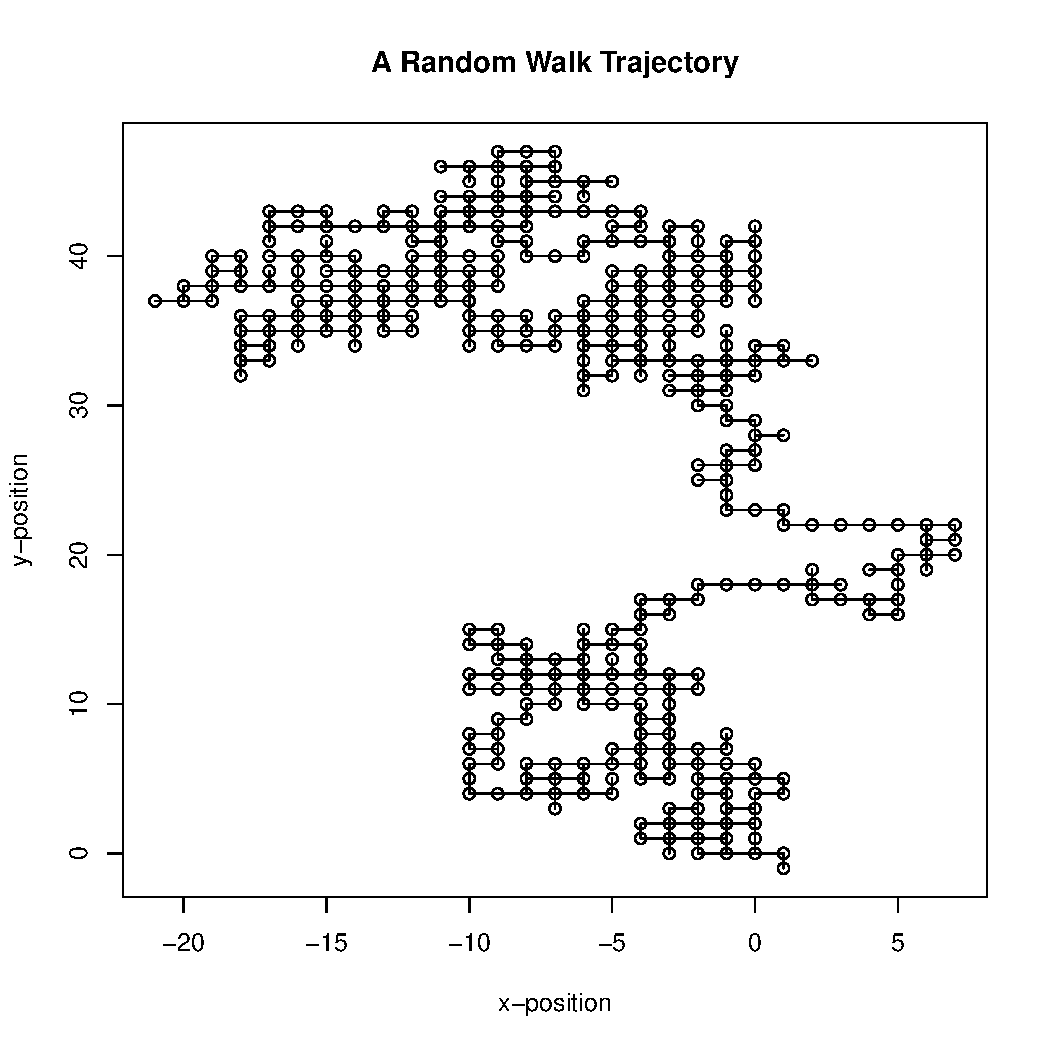
\includegraphics[width=\maxwidth]{figure/external-code-1-1} 
\begin{kframe}\begin{alltt}
\hlcom{# Change the start position}
\hlkwd{start}\hlstd{(my_walk)}\hlkwb{<-}\hlkwd{c}\hlstd{(}\hlnum{100}\hlstd{,}\hlnum{100}\hlstd{)}
\hlcom{# Plot AFTER we move the start}
\hlcom{# ...Hopefully they are the same shape, just shifted!}
\hlkwd{plot}\hlstd{(my_walk)}
\end{alltt}
\end{kframe}
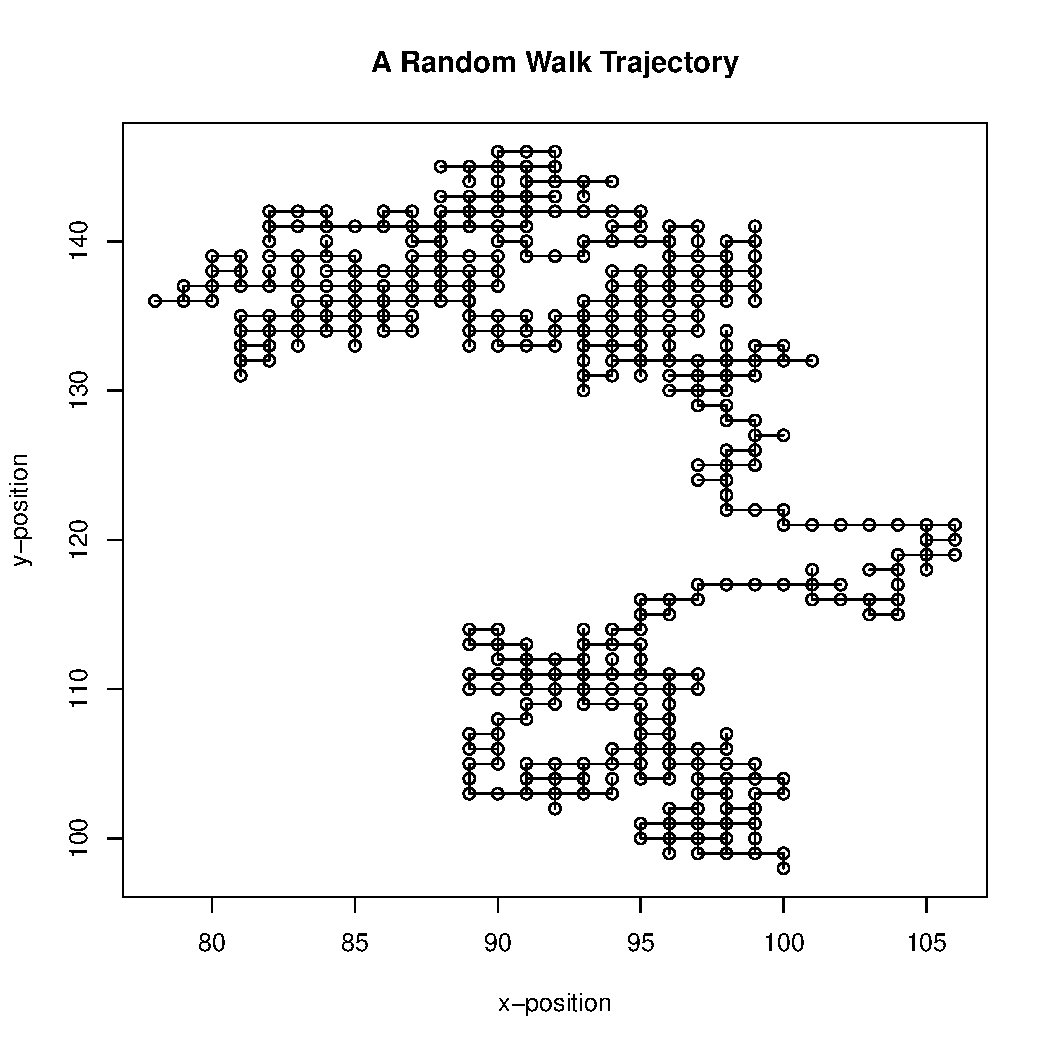
\includegraphics[width=\maxwidth]{figure/external-code-1-2} 
\begin{kframe}\begin{alltt}
\hlcom{# print the summary statistics}
\hlkwd{print}\hlstd{(my_walk)}
\end{alltt}
\begin{verbatim}
## [1] "Starting position:"
## [1] 100 100
## [1] "After this many steps...:"
## [1] 1000
## [1] "We arrive at:"
## [1] 144  94
\end{verbatim}
\end{kframe}
\end{knitrout}

\end{document}
